\chapter{Mixed action setup}%\addcontentsline{toc}{chapter}{Mixed action setup}

%%%%%%%%%%%%%%%%%%%%%%%%%%%%%%%%%%%%%%%%%%%%%%%%%%%%%%%%%%%
%%%%%%%%%%%%%%%%%%%%%%%%%%%%%%%%%%%%%%%%%%%%%%%%%%%%%%%%%%%
%%%%%%%%%%%%%%%%%%%%%%%%%%%%%%%%%%%%%%%%%%%%%%%%%%%%%%%%%%%
%%%%%%%%%%%%%%%%%%%%%%%%%%%%%%%%%%%%%%%%%%%%%%%%%%%%%%%%%%%

\label{ch_ma}

%%%%%%%%%%%%%%%%%%%%%%%%%%%%%%%%%%%%%%%%%%%%%%%%%%%%%%%%%%%
%%%%%%%%%%%%%%%%%%%%%%%%%%%%%%%%%%%%%%%%%%%%%%%%%%%%%%%%%%%
%%%%%%%%%%%%%%%%%%%%%%%%%%%%%%%%%%%%%%%%%%%%%%%%%%%%%%%%%%%
%%%%%%%%%%%%%%%%%%%%%%%%%%%%%%%%%%%%%%%%%%%%%%%%%%%%%%%%%%%

\section{Motivation}
\label{ch_ma:sec:introduction}

The lattice setup used in this is based on a mixed action with Wilson $\mathcal{O}(a)$ improved quarks (see Sec.~\ref{ch_foundation:subsec:Wilson}) in the sea and full twist Wilson tm quarks (see Sec.~\ref{ch_foundation:subsec:tm}) in the valence, the goal of which is to control cutoff effects associated with the heavy mass of the charm quark. These effects are of order $\mathcal{O}(am_c)$ with $m_c$ the mass of the charm quark. Exploiting automatic $\mathcal{O}(a)$ improvement of maximal twist Wilson tm fermions is expected to help in the control of the continuum limit and the mitigation of cutoff effects without the need to introduce any improvement coefficient in the charm sector. Furthermore, the mixed action is yet another valid lattice regularization which provides an independent way of measuring physical observables in the lattice. In this respect, it will allow us to quote independent precision results for the gradient flow scale $t_0$ (see Sec.~\ref{ch_ss}), the charm quark mass~\citep{charm} and the $D_{(s)}$ mesons decay constants~\citep{charm}.

For the definition of the mixed action approach, we recall eq.~(\ref{ch_foundation:eq:path_int})
\begin{align}
\left<O^{ij}(x_1)O^{ji}(x_2)\right>&=-\frac{1}{\mathcal{Z}}\int\mathcal{D}[U]e^{-S_{\textrm{G}}[U]-S_{\textrm{eff}}[U]}\times\\&{\textrm{tr}}\left(\Gamma D_i^{-1}(x_1,x_2)\Gamma D_j^{-1}(x_2,x_1)\right),\\
S_{\textrm{eff}}[U]&=-\sum_i^{N_f}\textrm{log det}(D_i).
\end{align} 
We see that the Dirac operator $D$ appears first in the Boltzmann factor $e^{-S_{\textrm{G}}[U]-S_{\textrm{eff}}[U]}$, which is referred to as the sea sector, with which the set of gauge ensembles is generated (see Appendix~\ref{appex_simulations}), and then in the fermionic observable whose expectation value we are interested in, which is referred to as the valence sector, thus appearing in two separate stages of the analysis: one the generation of gauge ensembles, the other the inversion of the Dirac operator on said gauge configurations (see Appendix~\ref{appex_solvers}). This in principle allows for the use of different regularizations of the Dirac operator in these two steps or sectors of the theory. This mixed action approach violates unitarity even once the continuum limit is taken unless the physical quark masses in both sea and valence coincide. This means that our setup will require a tuning procedure in which the values of the Wilson tm parameters are chosen in order to reproduce the same physical quark masses in the valence as in the sea sectors. This process is called matching of the mixed action. 

The flavor content of our setup is as follows. On the one hand, the sea sector has $N_f=2+1$ flavors, i.e. two mass-degenerate light quarks (corresponding to the $u$ and $d$ flavors) with mass $m_l$ and one strange quark with mass $m_s$. On the other hand, the valence sector consists of $N_f=2+1+1$ flavors, adding a charm quark. Since we have $N_f=2+1$ in the sea and $N_f=2+1+1$ in the valence, the flavors we need to match are the light and strange, treating the charm quark in the valence as a partially quenched flavor. 

In order to perform the matching of the theory, we need to know beforehand what values the physical quark masses take in the sea sector. This means that we need lattice measurements in the fully Wilson unitary setup (using the Wilson regularization in the sea and valence) in addition to the mixed action regularization. We therefore have two sets of data: those coming from the Wilson unitary setup, which we refer to as sea or Wilson results, and those coming from the mixed action itself. Using the two sets of data helps increasing the statistics of the scale setting analysis, as we will see in Sec.~\ref{ch_ss}. In addition to the matching of the sea and valence sectors, we also need to tune the valence action parameters to enforce full twist and automatic $\mathcal{O}(a)$ improvement.

The Chapter is structured as follows. In Sec.~\ref{ch_ma:sec:Sea} we discuss the sea sector details: ensembles under study, lattice actions and boundary conditions. In Sec.~\ref{ch_ma:sec:Valence} we discuss the valence sector, which employs Wilson tm quarks. In Sec.~\ref{ch_ma:sec:chiral_traj} we discuss the line of constant physics along which the ensembles under study were generated. They follow a chiral trajectory that suffers small mistunings and that must be corrected in order to go through the physical point. We discuss the details of a mass shifting procedure to account for these effects. Finally, in Sec.~\ref{ch_ma:sec:matching} we deal with the matching of sea and valence sectors though pseudoscalar masses in order to impose equal physical quark masses in both sectors and to recover unitarity in the continuum. We also explain the procedure to tune Wilson tm valence quarks to full twist.

%%%%%%%%%%%%%%%%%%%%%%%%%%%%%%%%%%%%%%%%%%%%%%%%%%%%%%%%%%%
%%%%%%%%%%%%%%%%%%%%%%%%%%%%%%%%%%%%%%%%%%%%%%%%%%%%%%%%%%%
%%%%%%%%%%%%%%%%%%%%%%%%%%%%%%%%%%%%%%%%%%%%%%%%%%%%%%%%%%%
%%%%%%%%%%%%%%%%%%%%%%%%%%%%%%%%%%%%%%%%%%%%%%%%%%%%%%%%%%%

\section{Sea sector}
\label{ch_ma:sec:Sea}

The gauge ensembles that we employ are CLS ensembles~\citep{Bruno:2014jqa,Mohler:2017wnb} with $N_f=2+1$ non-perturbatively $\mathcal{O}(a)$ improved Wilson fermions (see eq.~(\ref{ch_foundation:eq:DW_impr})). They use the Lüscher-Weisz gauge action~\citep{Luscher:1985zq}, which has reduced $\mathcal{O}(a^2)$ effects and is defined in eqs.~(\ref{ch_foundation:eq:SG_impr}-\ref{ch_foundation:eq:LW}).

For most of the ensembles, open boundary conditions (OBC) in time are used for the gauge fields, since it has been shown that with periodic boundary conditions (PBC) autocorrelations increase as one approaches the continuum limit, a problem known as critical slowing down. This is related to the existence of topological disconnected sectors in gauge field space, which avoids the algorithm to sample correctly different topological sectors. In contrast to this, OBC let the topological charge flow through the boundaries and topology freezing is thus avoided. All ensembles use PBC over the spatial volume.

The ensembles we consider have 5 different values of the lattice spacing, and for each of them there is one ensemble at the symmetric point, which is defined as $m_l=m_s$, or equivalently by the $\kappa$ parameter (see eq.~(\ref{ch_foundation:eq:kappa})) as $\kappa_l=\kappa_s$. All the ensembles, the complete list of which is shown in Table~\ref{apex_ensembles:tab:ens}, follow the chiral trajectory defined in eq.~(\ref{ch_ma:eq:chiral_traj}) below.


%%%%%%%%%%%%%%%%%%%%%%%%%%%%%%%%%%%%%%%%%%%%%%%%%%%%%%%%%%%
%%%%%%%%%%%%%%%%%%%%%%%%%%%%%%%%%%%%%%%%%%%%%%%%%%%%%%%%%%%
%%%%%%%%%%%%%%%%%%%%%%%%%%%%%%%%%%%%%%%%%%%%%%%%%%%%%%%%%%%
%%%%%%%%%%%%%%%%%%%%%%%%%%%%%%%%%%%%%%%%%%%%%%%%%%%%%%%%%%%


\section{Valence sector}
\label{ch_ma:sec:Valence}

In the valence sector, we employ a $N_f=2+1+1$ fully-twisted Wilson tm fermion action (see Sec.~\ref{ch_foundation:subsec:tm}), whose Dirac operator reads
\begin{equation}
D_{\textrm{W}}+\boldsymbol{m}^{\textrm{(v)}}+i\boldsymbol{\mu}^{\textrm{(v)}}\gamma_5,
\end{equation}
with 
\begin{gather}
\boldsymbol{\mu}^{\textrm{(v)}}={\textrm{diag}}(\mu_l,-\mu_l,-\mu_s,\mu_c)^{\textrm{(v)}}, \quad
\boldsymbol{m}^{\textrm{(v)}}={\textrm{diag}}(m_l,m_l,m_s,m_c)^{\textrm{(v)}}.
\end{gather}
In particular, we use the same standard quark mass for all flavors $m_l^{\textrm{(v)}}=m_s^{\textrm{(v)}}=m_c^{\textrm{(v)}}\equiv m^{\textrm{(v)}}$.

As discussed in Sec.~\ref{ch_foundation:subsec:tm}, to impose full twist means that the twist angles $\alpha_i$ fulfill
\begin{equation}
{\textrm{cot}}\;\alpha_i=\frac{m_i^{\textrm{R}}}{\mu_i^{\textrm{R}}}=0.
\end{equation}
To do so, it is enough to impose that the PCAC quark masses in eq.~(\ref{ch_observables:eq:PCAC}) vanish. When this is the case, automatic $\mathcal{O}(a)$ improvement of valence observables is obtained, up to cutoff effects coming from the sea sector due to the mixed action. However, these effects are expected to be $\mathcal{O}(g_0^4)$ in perturbation theory.

In order to find the valence parameters for which sea and valence physical quark masses are matched and full twist is obtained, we employ a grid of valence parameters values $\left(\kappa,\mu_l,\mu_s\right)^{\textrm{(v)}}$ around an estimate of the target point in order to perform small interpolations that allow us to find said target point $\left(\kappa,\mu_l,\mu_s\right)^{\textrm{(v)*}}$.

%%%%%%%%%%%%%%%%%%%%%%%%%%%%%%%%%%%%%%%%%%%%%%%%%%%%%%%%%%%
%%%%%%%%%%%%%%%%%%%%%%%%%%%%%%%%%%%%%%%%%%%%%%%%%%%%%%%%%%%
%%%%%%%%%%%%%%%%%%%%%%%%%%%%%%%%%%%%%%%%%%%%%%%%%%%%%%%%%%%
%%%%%%%%%%%%%%%%%%%%%%%%%%%%%%%%%%%%%%%%%%%%%%%%%%%%%%%%%%%

\section{Chiral trajectory}
\label{ch_ma:sec:chiral_traj}

The set of CLS ensembles that we use are generated along the trajectory in the quark mass plane defined by a constant trace of the bare sea ``(s)'' quark mass matrix
\begin{equation}
\label{ch_ma:eq:chiral_traj}
{\textrm{tr}}\left(M_q^{\textrm{(s)}}\right)=2m_l^{\textrm{(s)}}+m_s^{\textrm{(s)}}={\textrm{cnst}}.
\end{equation}
This trajectory ensures that at fixed lattice spacing the improved bare coupling 
\begin{equation}
\tilde{g}_0^2=g_0^2\left(1+ab_g{\textrm{tr}}\left(M_q^{\textrm{(s)}}\right)\right),
\end{equation}
is kept constant as we vary the sea quark masses to approach the physical point. Note that for the Wilson unitary setup, sea and valence quark masses are the same, but not for the mixed action setup. To ensure that this trajectory goes through the physical point, we define the dimensionless quantities
\begin{align}
\label{ch_ma:eq:phis}
\phi_2&=8t_0m_{\pi}^2,\\
\phi_4&=8t_0\left(m_K^2+\frac{1}{2}m_{\pi}^2\right),
\end{align}
which to LO ChPT are proportional to the renormalized quark masses
\begin{align}
\phi_2&\propto m_l^{\textrm{R}},\\
\phi_4&\propto2m_l^{\textrm{R}}+m_s^{\textrm{R}}={\textrm{tr}}\left(M_q^{\textrm{R}}\right).
\end{align}
The trace of the renormalized quark mass matrix ${\textrm{tr}}\left(M_q^{\textrm{R}}\right)$ is in turn proportional to the bare quark mass matrix up to $\mathcal{O}(a)$ cutoff effects
\begin{equation}
{\textrm{tr}}\left(M_q^{\textrm{R}}\right)=Z_mr_m\left[\left(1+a\bar{d}_m{\textrm{tr}}\left(M_q\right)\right){\textrm{tr}}\left(M_q\right)+ad_m{\textrm{tr}}\left(M_q^2\right)\right].
\end{equation}
Thus, setting the sea value of $\phi_4$ to its physical value for all ensembles ensure that eq.~(\ref{ch_ma:eq:chiral_traj}) holds and goes through the physical point, up to small mistunings due to higher terms in the chiral expansion and to cutoff effects. 

To correct for these mistunings, we perform small mass shifts~\citep{Bruno:2016plf} in the bare sea quark masses by Taylor expanding lattice observables as
\begin{equation}
\label{ch_ma:eq:mass_shift}
{O}\left(m_l^{\textrm{(s)'}},m_s^{\textrm{(s)'}}\right)={O}\left(m_l^{\textrm{(s)}},m_s^{\textrm{(s)}}\right)+\sum_q\left(m_q^{\textrm{(s)'}}-m_q^{\textrm{(s)}}\right)\frac{d{O}}{dm_q^{\textrm{(s)}}},
\end{equation}
with the total derivative given by
\begin{equation}
\label{ch_ma:eq:md}
\frac{d{O}}{dm_q^{\textrm{(s)}}}=\sum_i\frac{\partial{O}}{\partial \left<P_i\right>}\left[\left<\frac{\partial P_i}{\partial m_q^{\textrm{(s)}}}\right>-\left<P_i\frac{\partial S}{\partial m_q^{\textrm{(s)}}}\right>+\left<P_i\right>\left<\frac{\partial S}{\partial m_q^{\textrm{(s)}}}\right>\right].
\end{equation}
Here ${O}$ is an arbitrary lattice observable and $\{P_i\}_{i=1,2,...}$ is the set of primary observables on which it depends, in our case the corresponding two-point functions. The first term in the right hand side of this equation corresponds to the valence contribution to the derivative, while the other terms correspond to the sea contributions. Note that for the Wilson unitary setup, all terms contribute, while for the mixed action setup, since the two-point functions $\{P_i\}$ do not depend explicitly on $m_q^{\textrm{(s)}}$, the first term in the right hand side of eq.~(\ref{ch_ma:eq:md}) vanishes.

In particular the sum over $q$ in eq.~(\ref{ch_ma:eq:mass_shift}) can be done in any direction of the quark mass plane, and following~\citep{Strassberger:2021tsu} we choose to mass shift only the strange quark. For practical purposes, since we want to mass shift all relevant observables for each ensemble to satisfy that the sea value of $\phi_4$ is equal to its physical value, $\phi_4^{\textrm{(s)}}=\phi_4^{\textrm{ph}}={\textrm{const.}}$, following~\citep{Strassberger:2023xnj} we rewrite the Taylor expansion as
\begin{equation}
{O}\left(\phi_4^{\textrm{(s)'}}=\phi_4^{\textrm{ph}}\right)={O}\left(\phi_4^{\textrm{(s)}}\right)+\left(\phi_4^{\textrm{ph}}-\phi_4^{\textrm{(s)}}\right)\frac{d{O}}{d\phi_4^{\textrm{(s)}}},
\end{equation}
with
\begin{equation}
\frac{d{O}}{d\phi_4^{\textrm{(s)}}}=\frac{d{O}/dm_s^{\textrm{(s)}}}{d\phi_4^{\textrm{(s)}}/dm_s^{\textrm{(s)}}}.
\end{equation}
Note that by the sea value $\phi_4^{\textrm{(s)}}$ we refer to $\phi_4$ computed in the Wilson unitary setup, and its derivative has both sea and valence contributions, while $d{O}/dm_s^{\textrm{(s)}}$ has valence and sea contributions when the observable ${O}$ is computed in the Wilson unitary setup, and only sea contributions when ${O}$ is computed in the mixed action regularization. In the Wilson unitary setup, imposing $\phi_4^{\textrm{(s)}}=\phi_4^{\textrm{ph}}={\textrm{const.}}$ means that so does the valence value of $\phi_4$, while for the mixed action regularization this is not true. In this case in addition to fixing $\phi_4^{\textrm{(s)}}=\phi_4^{\textrm{ph}}={\textrm{const.}}$ with the mass shifting procedure we need later to impose $\phi_4^{\textrm{(v)}}=\phi_4^{\textrm{(s)}}$, which is done through the matching between sea and valence sectors (see Sec.~\ref{ch_ma:sec:matching}).

The observables we will be interested for the scale setting (see Sec.~\ref{ch_ss}) are $\sqrt{t_0}f_{\pi}$, $\sqrt{t_0}f_{K}$ and $\sqrt{t_0}f_{\pi K}$, the latter defined in eq.~(\ref{ch_ss:eq:fpik}). We also include the derivatives of $\sqrt{t_0}m_{12}^{\textrm{R}}$ in the mixed action setup since we will need to mass shift this quantity in order to tune to full twist (see Sec.~\ref{ch_ma:sec:matching}). All these quantities are physical and so are their derivatives with respect to $\phi_4$. Thus, one can measure these derivatives for each ensemble and then fit them as a function of $\phi_2$ and the lattice spacing. This allows to evaluate the result of these fits at the values of $\phi_2$ and $t_0/a^2$ corresponding to each ensemble and perform the mass shift with that result instead of using the individual measurements of each ensemble. This has the advantage of improving the precision for observables whose mass derivatives are noisy or missing, which is particularly relevant for the finest lattice spacing and the most chiral ensembles under study.

For fitting the derivatives we use
\begin{equation}
\label{ch_ma:eq:md_1}
F=A+B\phi_2+D\frac{a^2}{t_0},
\end{equation}
for all choices of ${O}$ except for the light PCAC quark mass in the mixed action setup, for which we use
\begin{equation}
\label{ch_ma:eq:md_2}
F=A+B\phi_2+C\phi_2^2+(D+E\phi_2)\frac{a^2}{t_0},
\end{equation}
for empirical reasons.

In the case of $\phi_2$ in the Wilson regularization, we exclude the symmetric point ensembles from the fit of its mass derivative, since $\phi_2^{\textrm{sym}}=\frac{2}{3}\phi_4$ by construction. Thus, for these ensembles we will use this relation directly to mass shift $\phi_2$.

Results for the fit parameters are presented in Table~\ref{ch_ma:tab:md}, while plots are shown in Figs.~\ref{ch_ma:fig:dfpik_w}-\ref{ch_ma:fig:dphi4_tm}.

We have assumed knowledge of the physical value of $\phi_4$ to which we mass shift all ensembles. However, in order to determine it we need the physical value of the intermediate scale $t_0$, which is the target of the analysis. Thus, we start the process with an educated guess of $t_0^{\textrm{ph}}$, which provides with an initial guess for $\phi_4^{\textrm{ph}}$. Once the scale setting has been done and a new determination of $t_0^{\textrm{ph}}$ is obtained, the analysis is iterated, updating the value of $\phi_4^{\textrm{ph}}$ to which the ensembles are shifted, until convergence is observed in this observable. The initial guess used for $t_0^{\textrm{ph,\;guess}}$ is just a number with no error. After a few iterative steps of the analysis, we obtain the new estimate
\begin{equation}
\label{ch_ma:eq:t0_guess}
t_0^{\textrm{ph,\;guess}}=0.1445(6),
\end{equation}
where the uncertainty keeps all the correlations with the lattice data entering the analysis. Eq.~(\ref{ch_ma:eq:t0_guess}) determines the value of $\phi_4^{\textrm{ph}}$ to which we perform the mass shifts in the subsequent sections, the input values for physical $m_{\pi}$ and $m_K$ given in eq.~(\ref{ch_ss:eq:isoQCD}). 

\begin{longtable}{c | c c c c c}
\label{ch_ma:tab:md}
    ${O}$ & A & B & C & D & E \\
    \toprule
    $\sqrt{t_0}f_{\pi K}^{\textrm{W}}$ & 0.017(8) & -0.007(10) & - & 0.024(26) & - \\ 
    $\sqrt{t_0}f_{\pi}^{\textrm{W}}$ & 0.006(8) & 0.008(9) & - & 0.020(26) & - \\ 
    $\sqrt{t_0}f_{K}^{\textrm{W}}$ & 0.024(10) & -0.016(11) & - & 0.022(27) & - \\ 
    $\phi_2^{\textrm{W}}$ & 0.004(36) & 0.131(92) & - & 0.874(129) & - \\ 
    $t_0$ & -0.437(84) & 0.214(101) & - & -0.264(274) & - \\ 
    \midrule
    $\sqrt{t_0}f_{\pi K}^{\textrm{tm}}$ & -0.009(7) & 0.011(8) & - & -0.014(18) & - \\ 
    $\sqrt{t_0}f_{\pi}^{\textrm{tm}}$ & -0.007(6) & 0.013(8) & - & -0.028(18) & - \\ 
    $\sqrt{t_0}f_{K}^{\textrm{tm}}$ & -0.009(8) & 0.010(10) & - & -0.006(18) & - \\ 
    $\sqrt{t_0}m_{12}^{\textrm{tm, R}}$ & -0.004(3) & 0.035(10) & -0.041(9) & 0.020(16) & 0.026(24) \\ 
    $\phi_2^{\textrm{tm}}$ & 0.031(17) & -0.032(23) & - & -0.102(73) & - \\ 
    $\phi_4^{\textrm{tm}}$ & 0.006(37) & 0.050(47) & - & -0.298(126) & - \\ 
    \bottomrule
    \caption{Results for the fit parameters in eqs.~(\ref{ch_ma:eq:md_1}-\ref{ch_ma:eq:md_2}) for the lattice observables that will be used in the analysis. The superscript ``W'' refers to the observable being computed in the Wilson unitary setup, while ``tm'' refers to the mixed action setup.}
\end{longtable}

\begin{figure}
    \centering
    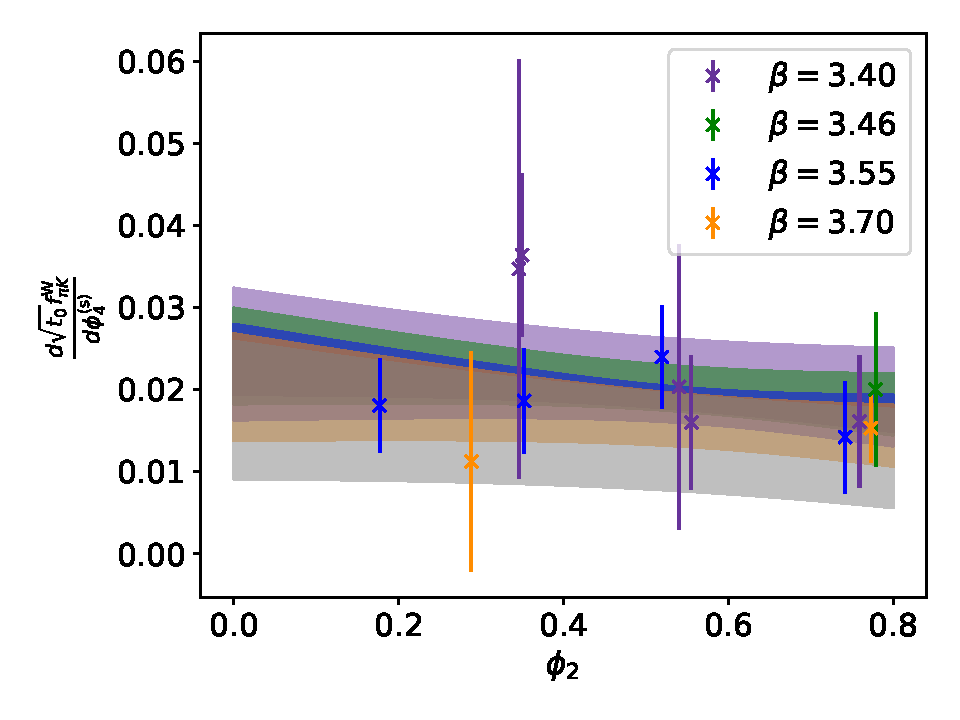
\includegraphics[width=1.\textwidth]{./cap4/figs/dt0fpik_w.pdf}
    \caption{Derivative $d\sqrt{t_0}f_{\pi K}/d\phi_4^{\textrm{(s)}}$ for the Wilson unitary setup. For the fit eq.~(\ref{ch_ma:eq:md_1}) was used. Results for the fit parameters are presented in Table~\ref{ch_ma:tab:md}.}
    \label{ch_ma:fig:dfpik_w}
\end{figure}

\begin{figure}
    \centering
    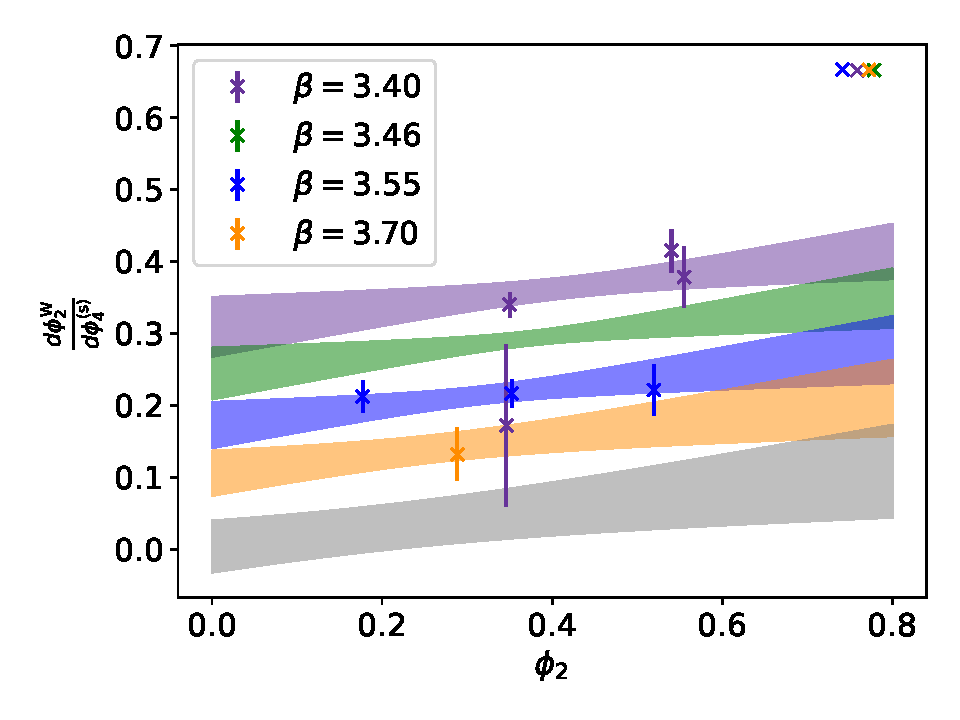
\includegraphics[width=1.\textwidth]{./cap4/figs/dphi2_w.pdf}
    \caption{Derivative $d\phi_2/d\phi_4^{\textrm{(s)}}$ for the Wilson unitary setup. For the fit eq.~(\ref{ch_ma:eq:md_1}) was used. Results for the fit parameters are presented in Table~\ref{ch_ma:tab:md}.}
    \label{ch_ma:fig:dphi2_w}
\end{figure}

\begin{figure}
    \centering
    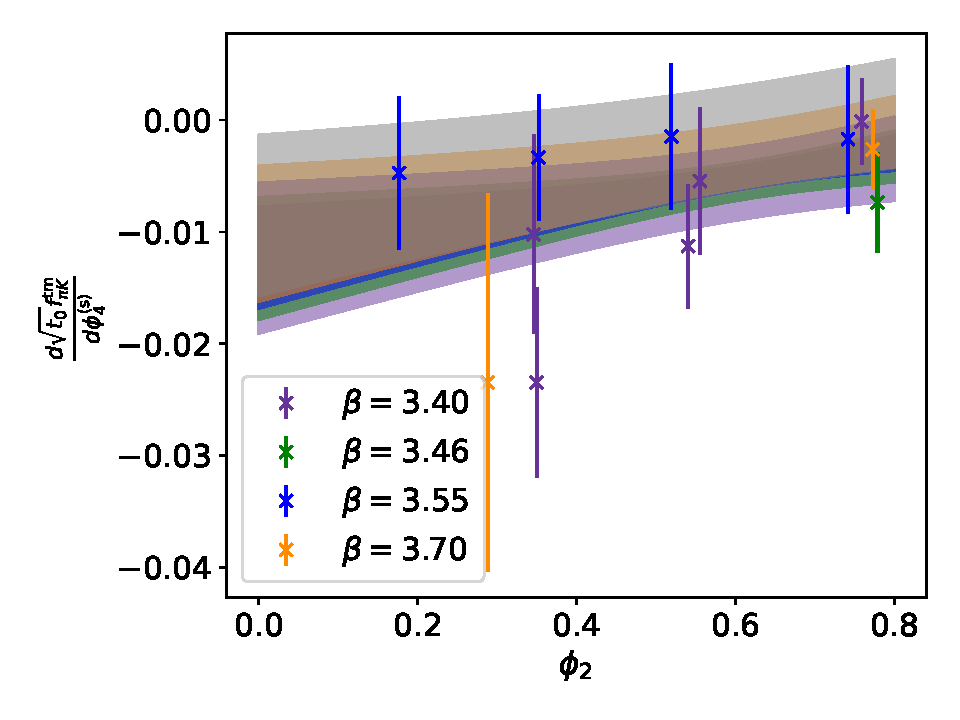
\includegraphics[width=1.\textwidth]{./cap4/figs/dt0fpik_tm.pdf}
    \caption{Derivative $d\sqrt{t_0}f_{\pi K}/d\phi_4^{\textrm{(s)}}$ for the mixed action setup. For the fit eq.~(\ref{ch_ma:eq:md_1}) was used. Results for the fit parameters are presented in Table~\ref{ch_ma:tab:md}.}
    \label{ch_ma:fig:dfpik_tm}
\end{figure}

\begin{figure}
    \centering
    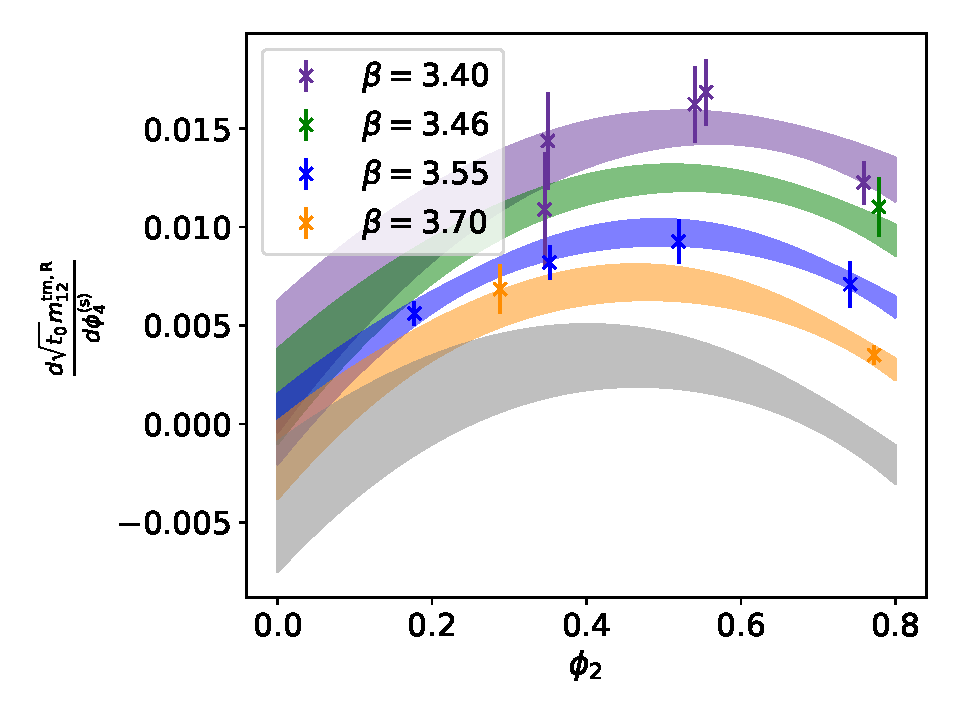
\includegraphics[width=1.\textwidth]{./cap4/figs/dt0m12_tm.pdf}
    \caption{Derivative $d\sqrt{t_0}m_{12}^{\textrm{R}}/d\phi_4^{\textrm{(s)}}$ for the mixed action setup. For the fit eq.~(\ref{ch_ma:eq:md_2}) was used. Results for the fit parameters are presented in Table~\ref{ch_ma:tab:md}.}
    \label{ch_ma:fig:dm12_tm}
\end{figure}

\begin{figure}
    \centering
    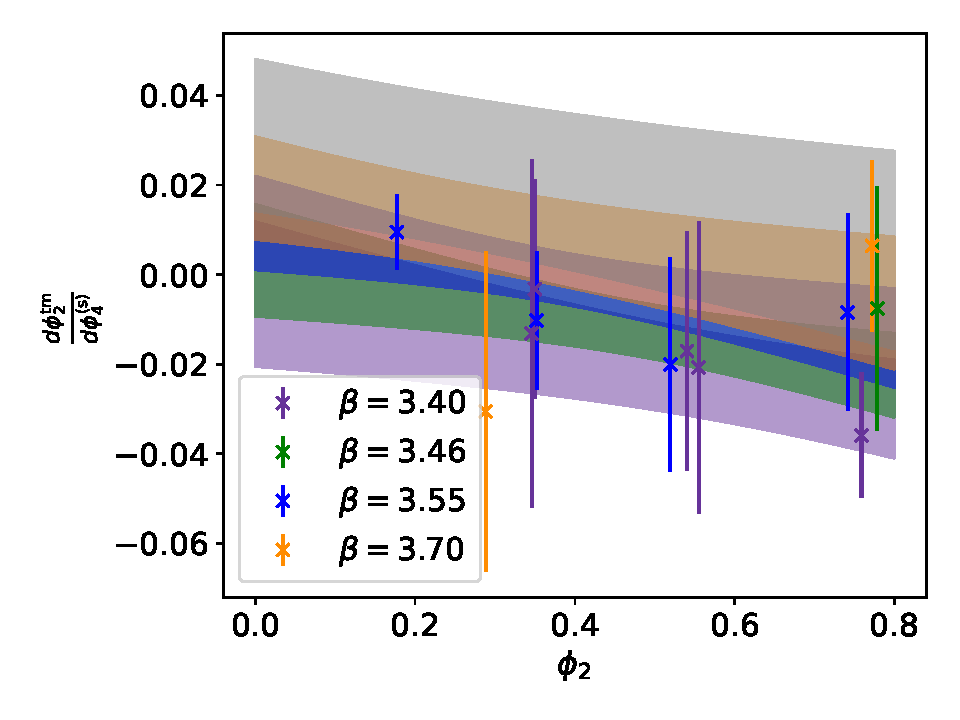
\includegraphics[width=1.\textwidth]{./cap4/figs/dphi2_tm.pdf}
    \caption{Derivative $d\phi_2/d\phi_4^{\textrm{(s)}}$ for the mixed action setup. For the fit eq.~(\ref{ch_ma:eq:md_1}) was used. Results for the fit parameters are presented in Table~\ref{ch_ma:tab:md}.}
    \label{ch_ma:fig:dphi2_tm}
\end{figure}

\begin{figure}
    \centering
    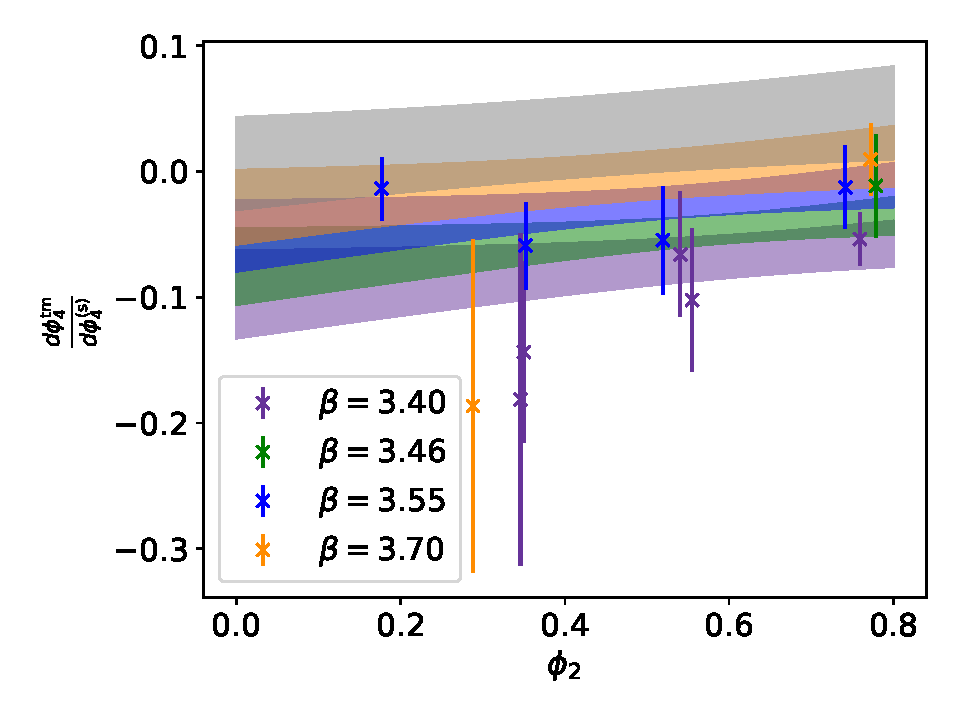
\includegraphics[width=1.\textwidth]{./cap4/figs/dphi4_tm.pdf}
    \caption{Derivative $d\phi_4/d\phi_4^{\textrm{(s)}}$ for the mixed action setup. For the fit eq.~(\ref{ch_ma:eq:md_1}) was used. Results for the fit parameters are presented in Table~\ref{ch_ma:tab:md}.}
    \label{ch_ma:fig:dphi4_tm}
\end{figure}

%%%%%%%%%%%%%%%%%%%%%%%%%%%%%%%%%%%%%%%%%%%%%%%%%%%%%%%%%%%
%%%%%%%%%%%%%%%%%%%%%%%%%%%%%%%%%%%%%%%%%%%%%%%%%%%%%%%%%%%
%%%%%%%%%%%%%%%%%%%%%%%%%%%%%%%%%%%%%%%%%%%%%%%%%%%%%%%%%%%
%%%%%%%%%%%%%%%%%%%%%%%%%%%%%%%%%%%%%%%%%%%%%%%%%%%%%%%%%%%


\section{Matching and tuning to full twist}
\label{ch_ma:sec:matching}

As explained in Sec.~\ref{ch_ma:sec:Valence}, when working with a mixed action, after performing the mass shifts in Sec.~\ref{ch_ma:sec:chiral_traj}, we need to match the physical quark masses of the sea and valence sectors. To do this, we use a grid of valence parameter values to find the target point with small interpolations. In order to know the values of the relevant observables in the sea, we use measurements in the fully Wilson unitary setup.
In practice, to compute the physical quark masses we need the relevant improvement coefficients. In order not to rely on these for the matching procedure, instead of matching the physical quark masses we choose to use the pion and kaon masses in units of the gradient flow scale $t_0$
\begin{align}
\label{ch_ma:eq:matching}
\phi_2^{\textrm{(s)}}&=\phi_2^{\textrm{(v)}},\\
\phi_4^{\textrm{(s)}}&=\phi_4^{\textrm{(v)}}.
\end{align}
since these quantities are proportional to the physical quark masses to LO ChPT (see eq.~(\ref{ch_ma:eq:phis})).

In addition to this, we need to tune the Wilson tm action to full twist, which means setting the valence PCAC quark mass to zero
\begin{equation}
\label{ch_ma:eq:full-twist}
m_{ud}^{\textrm{(v)}}\equiv m_{ll'}^{\textrm{(v)}}\equiv m_{12}^{\textrm{(v)}}=0.
\end{equation}
In principle, we should also set the strange PCAC quark mass to zero. However, since the $\kappa^{\textrm{(v)}}$ parameter we use is flavor degenerate, this condition is automatically satisfied (up to cutoff effects) once eq.~(\ref{ch_ma:eq:full-twist}) is imposed.

To impose eqs.~(\ref{ch_ma:eq:matching}-\ref{ch_ma:eq:full-twist}), we perform interpolations of the valence observables $m_{12}^{\textrm{(v)}},\phi_2^{\textrm{(v)}},\phi_4^{\textrm{(v)}}$ in the $\left(\kappa,\mu_l,\mu_s\right)^{\textrm{(v)}}$ hyperplane, using as fit functions the following expressions motivated by ChPT
\begin{align}
m_{12}^{\textrm{(v)}}&=p_1\left(\frac{1}{\kappa^{\textrm{(v)}}}-\frac{1}{\kappa^{\textrm{(v)*}}}\right)+p_2\left(\mu_l^{\textrm{(v)}}-\mu_l^{\textrm{(v)*}}\right),\\
\phi_2^{\textrm{(v)}}&=\frac{p_3}{\mu_l^{\textrm{(v)}}}\left(\frac{1}{\kappa^{\textrm{(v)}}}-\frac{1}{\kappa^{\textrm{(v)*}}}\right)^2+p_4\left(\mu_l^{\textrm{(v)}}-\mu_l^{\textrm{(v)*}}\right)+\phi_2^{\textrm{(s)}},\\
\phi_4^{\textrm{(v)}}&=\frac{p_5}{\mu_l^{\textrm{(v)}}}\left(\frac{1}{\kappa^{\textrm{(v)}}}-\frac{1}{\kappa^{\textrm{(v)*}}}\right)^2+\frac{p_6}{\mu_s^{\textrm{(v)}}}\left(\frac{1}{\kappa^{\textrm{(v)}}}-\frac{1}{\kappa^{\textrm{(v)*}}}\right)^2 \\
&+p_7\left(\mu_l^{\textrm{(v)}}-\mu_l^{\textrm{(v)*}}\right)+p_8\left(\mu_s^{\textrm{(v)}}-\mu_s^{\textrm{(v)*}}\right)+\phi_4^{\textrm{(s)}}.
\end{align}
This way, the target point values $\left(\kappa,\mu_l,\mu_s\right)^{\textrm{(v)*}}$ are found as fit parameters. The interpolation is shown in Fig.~\ref{ch_ma:fig:match}. A simultaneous fit of these three quantities is performed.

The mixed action results for the quark masses are given exactly by the target twist mass parameters $\mu_{l,s}^{\textrm{(v)*}}$, while the extraction of the pion and kaon decay constants in the mixed action setup requires an additional interpolation along the valence grid to the target point. The fit functions for this interpolation are
\begin{align}
f_{\pi}^{\textrm{(v)}}&=q_1\left(\frac{1}{\kappa^{\textrm{(v)}}}-\frac{1}{\kappa^{\textrm{(v)*}}}\right)^2+q_2\left(\frac{1}{\kappa^{\textrm{(v)}}}-\frac{1}{\kappa^{\textrm{(v)*}}}\right)+q_3\mu_l^{\textrm{(v)}},\\
f_K^{\textrm{(v)}}&=r_1\left(\frac{1}{\kappa^{\textrm{(v)}}}-\frac{1}{\kappa^{\textrm{(v)*}}}\right)^2+r_2\left(\frac{1}{\kappa^{\textrm{(v)}}}-\frac{1}{\kappa^{\textrm{(v)*}}}\right)+r_3\mu_l^{\textrm{(v)}}+r_4\mu_s^{\textrm{(v)}}.
\end{align}
The interpolation for the decay constants combination $f_{\pi K}$ defined in eq.~(\ref{ch_ss:eq:fpik}) is shown in Fig.~\ref{ch_ma:fig:fpik_interp}.

\begin{figure}
    \centering
    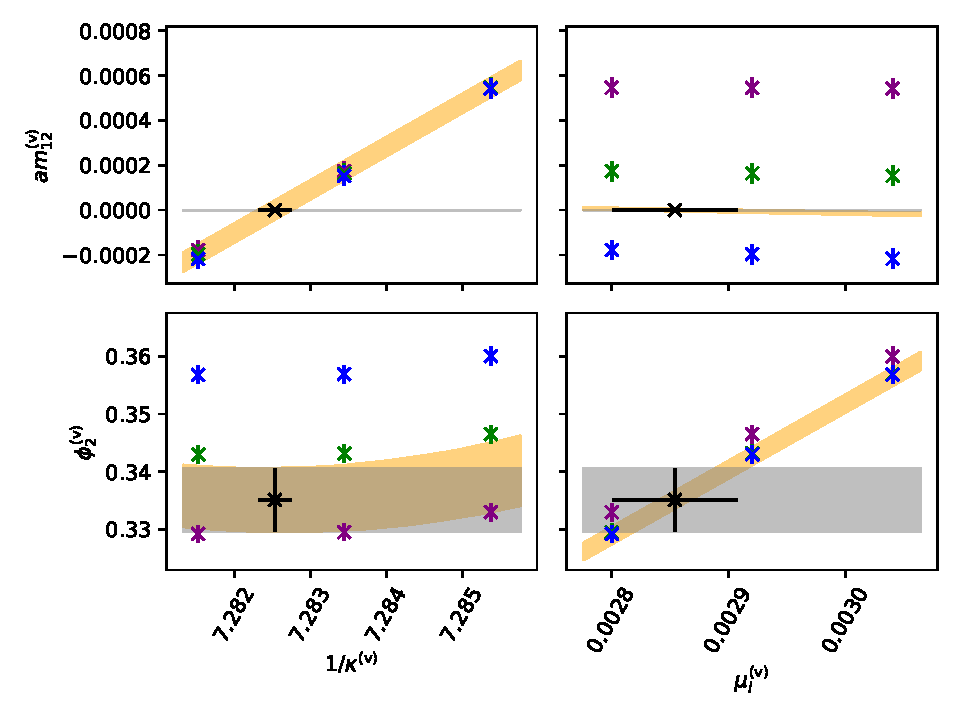
\includegraphics[width=1.\textwidth]{./cap4/figs/matching_H105.pdf}
    \caption{Plot of the matching of sea (gray band) and valence values of $\phi_2$ and tuning to full twist $am_{12}^{\textrm{(v)}}=0$ along the grid of valence parameters values. Each point represents a different measurement in the valence along the grid, and the orange band represents the interpolation. The black point is the target result $\left(\kappa,\mu_l,\mu_s\right)^{\textrm{(v)*}}$. Here we only show the matching of $\phi_2^{\textrm{(v)}}$ and $am_{12}^{\textrm{(v)}}$, though the matching of $\phi_4^{\textrm{(v)}}$ is done simultaneously. Ensemble is H105.}
    \label{ch_ma:fig:match}
\end{figure}

\begin{figure}
    \centering
    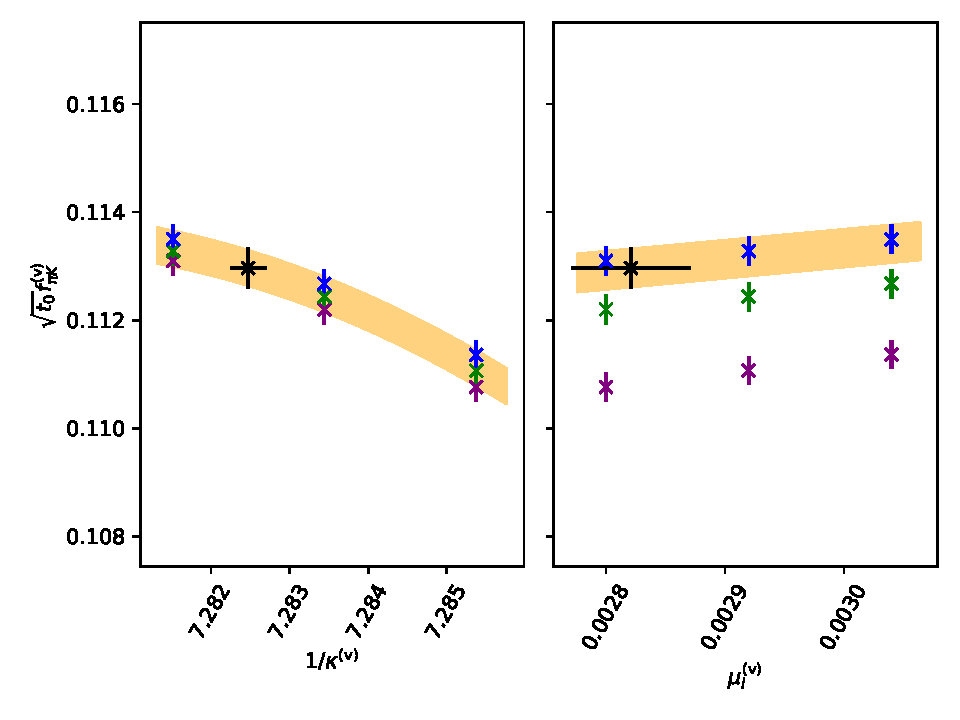
\includegraphics[width=1.\textwidth]{./cap4/figs/interp_fpik_H105.pdf}
    \caption{Interpolation of $\sqrt{t_0}f_{\pi K}$ (see eq.~(\ref{ch_ss:eq:fpik})) along the valence grid to the target point $\left(\kappa,\mu_l,\mu_s\right)^{\textrm{(v)*}}$. The points with different colors represent measurements at different values of the valence parameters. Ensemble is H105.}
    \label{ch_ma:fig:fpik_interp}
\end{figure}

%%%%%%%%%%%%%%%%%%%%%%%%%%%%%%%%%%%%%%%%%%%%%%%%%%%%%%%%%%%
%%%%%%%%%%%%%%%%%%%%%%%%%%%%%%%%%%%%%%%%%%%%%%%%%%%%%%%%%%%
%%%%%%%%%%%%%%%%%%%%%%%%%%%%%%%%%%%%%%%%%%%%%%%%%%%%%%%%%%%
%%%%%%%%%%%%%%%%%%%%%%%%%%%%%%%%%%%%%%%%%%%%%%%%%%%%%%%%%%%
